\documentclass[10pt]{article}
\usepackage[utf8]{inputenc}
\usepackage[T1]{fontenc}
\usepackage{amsmath}
\usepackage{amsfonts}
\usepackage{amssymb}
\usepackage[version=4]{mhchem}
\usepackage{stmaryrd}
\usepackage{graphicx}
\usepackage[export]{adjustbox}
\graphicspath{ {./images/} }

\begin{document}

    (T12.1) A black hole ( BH ) typically forms by the gravitational collapse of a massive star at the end of its life cycle to a point called a singularity. Due to the extreme gravity of such an object, nothing that enters the so-called event horizon (a spherical surface with $r=R_{\mathrm{SC}}$, where $r$ is the distance from the singularity) is able to escape from it. Here, $R_{\mathrm{SC}}$ is referred to as the Schwarzschild radius.\\
    (T12.1a) Modelling the origin of Hawking radiation: Consider a pair of particles, each with mass $m$ , produced on either side of the BH horizon. One particle is slightly outside the horizon at $r \approx R_{\mathrm{SC}}$, while the other particle is inside the horizon at $r=\kappa R_{\mathrm{SC}}$. Assume that the total energy of a particle is the sum of its rest mass energy $m c^{2}$ and the gravitational potential energy due to the BH .
    
    Determine the value of $\kappa$ for which the particle pair has zero total energy.\\
    (T12.1b) Temperature of a black hole: If the particle produced outside the horizon in the above process has enough kinetic energy, it may escape the BH in a process called Hawking radiation. The one inside the horizon, which has negative energy, gets absorbed and decreases the mass of the BH.
    
    Assume that all Hawking radiation is made of photons with a black body spectrum which peaks at the wavelength $\lambda_{\mathrm{bb}} \approx 16 R_{\mathrm{SC}}$. It is known that for a solar mass BH , $R_{\mathrm{SC}, \odot}=2.952 \mathrm{~km}$.
    
    Obtain an expression for the temperature, $T_{\mathrm{bh}}$, of the BH corresponding to this black body radiation, in terms of its mass $M_{\mathrm{bh}}$ and physical constants. Calculate the Schwarzschild radius, $R_{\mathrm{SC}, 10 \odot}$, and temperature, $T_{\mathrm{bh}, 10 \odot}$, for a BH with mass $10 \mathrm{M}_{\odot}$.\\
    (T12.1c) Mass loss of a black hole: Assume that the Hawking radiation is emitted out from the event horizon.
    
    Using the mass-energy equivalence, obtain an expression for the rate of mass loss, $d M_{\mathrm{bh}}(t) / d t$, in terms of the mass $M_{\mathrm{bh}}(t)$ of the BH and physical constants.
    
    Hence, obtain an expression for $M_{\mathrm{bh}}(t)$ for a BH with initial mass $M_{0}$. Sketch $M_{\mathrm{bh}}(t)$ as a function of $t$ from $M_{\mathrm{bh}}=M_{0}$ to $M_{\mathrm{bh}}=0$.\\
    (T12.1d) Lifetime of a black hole: Obtain an expression for the lifetime $\tau_{\mathrm{BH}}$ at which a black hole with initial mass $M_{0}$ completely evaporates due to Hawking radiation, in terms of $M_{0}$ and physical constants. Calculate the lifetime $\tau_{\mathrm{bh}, 10 \odot}$ (in seconds) for a black hole with $M_{0}=10 \mathrm{M}_{\odot}$.\\
    (T12.1e) Black hole in a CMB radiation bath: Consider an isolated black hole in space, far away from other bodies, with a current temperature $T_{\mathrm{bh}}^{\text {now }}$, surrounded by the cosmic microwave background (CMB) with a current temperature $T_{\mathrm{cmb}}^{\text {now }}=2.7 \mathrm{~K}$. The black hole can grow in mass by absorbing CMB radiation, and lose its mass by Hawking radiation.
    
    Taking into account the accelerating expansion of the Universe, identify which of the following figures show the long-term time evolution of $T_{\mathrm{bh}}$ in the following three cases: (X) $T_{\mathrm{bh}}^{\mathrm{now}}>T_{\mathrm{cmb}}^{\mathrm{now}}$, (Y) $T_{\mathrm{bh}}^{\mathrm{now}}=T_{\mathrm{cmb}}^{\mathrm{now}}$, (Z) $T_{\mathrm{bh}}^{\mathrm{now}}<T_{\mathrm{cmb}}^{\mathrm{now}}$.

    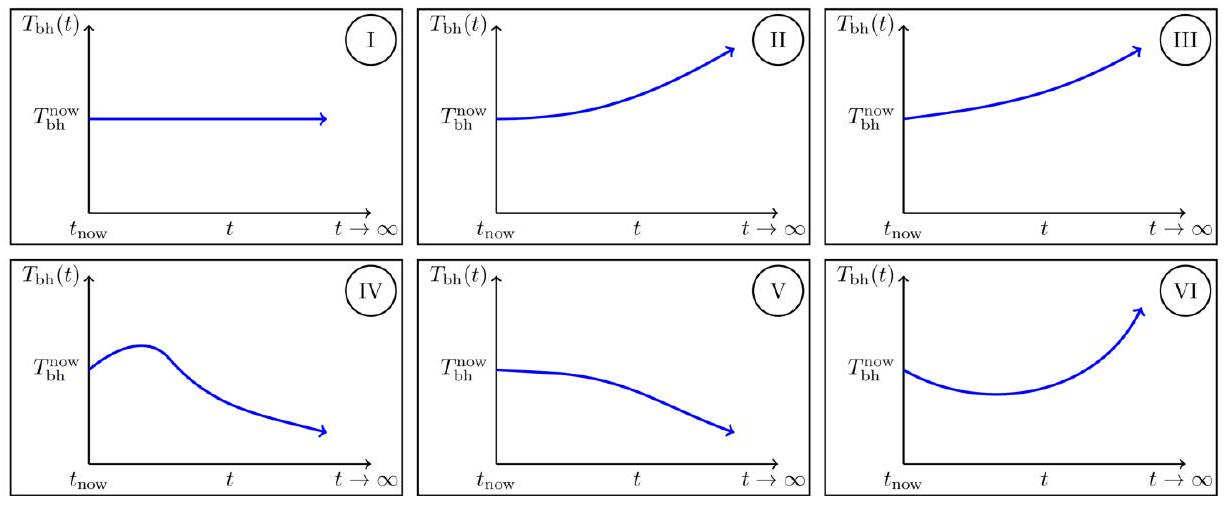
\includegraphics[max width=\textwidth, center]{2025_08_23_e94579452776a99c4850g-18}
    
    Indicate your answer by ticking the appropriate box (only one) for each case $\mathrm{X}, \mathrm{Y}$ or Z in the Table given in the Summary Answersheet corresponding to the appropriate figure number.\\
    (T12.2) Primordial black holes (PBHs) of much smaller masses can form in the very early Universe. All the following questions are related to PBHs. Here, any processes that increase the mass of the black hole may be neglected.\\
    (T12.2a) PBH evaporating at the current epoch: As you may have noticed from the answers to the previous questions, black holes of solar mass would take a long time to evaporate. However, since PBHs can have a much smaller mass, we may be able to see them evaporating in current times.
    
    Find the initial mass $M_{0, \mathrm{PBH}}$ (in kg), Schwarzschild radius $R_{\mathrm{SC}, \mathrm{PBH}}$ (in m), and temperature $T_{\mathrm{PBH}}$ (in K) of a black hole that may be evaporating away completely at the present epoch, i.e., those with lifetime $\tau_{\mathrm{PBH}}=14$ billion years.\\
    (T12.2b) Formation of a PBH: In the radiation-dominated early Universe, the scale factor varies as $a(t) \sim t^{1 / 2}$. In this era, PBHs form due to the collapse of all energy contained in a region of physical size $c t$, where $t$ is the age of the Universe at that time.
    
    A PBH with mass of $1 \times 10^{12} \mathrm{~kg}$ forms when the age of the Universe is about $1 \times 10^{-23} \mathrm{~s}$. Calculate the age of the Universe, $t_{20}$, when a PBH of mass $1 \times 10^{20} \mathrm{~kg}$ forms.\\
    (T12.2c) Observed spectrum of Hawking radiation from PBH: Consider a PBH of initial mass $1 \times 10^{10} \mathrm{~kg}$ which completely evaporates at the end of its lifetime $\tau_{\mathrm{PBH}}$. For this part, assume for simplicity that most of the Hawking radiation is emitted at this time, with a temperature corresponding to its initial mass. Also, take the scale factor of the Universe to be evolving as $a(t) \sim t^{2 / 3}$.
    
    Calculate the peak wavelength of this Hawking radiation as observed at Earth, $\lambda_{\text {earth }}$, at the present epoch (at $t=14$ billion years).\\
    (T12.2d) High energy cosmic radiation from PBH: Now assume that the Hawking radiation emitted at a given time $t$ corresponds to photons emitted with an energy $k_{\mathrm{B}} T_{\mathrm{bh}}(t)$. Also, the highest possible temperature for a black hole is the Planck temperature $T_{\text {Planck }}$ where $k_{\mathrm{B}} T_{\text {Planck }}=1 \times 10^{19} \mathrm{GeV}$.
    
    The evolution of the scale factor over relevant time scales is given in the following figure. The scale factor today is set to be unity. $t(s)$ on the time axis represents the age of the universe in seconds.\\
    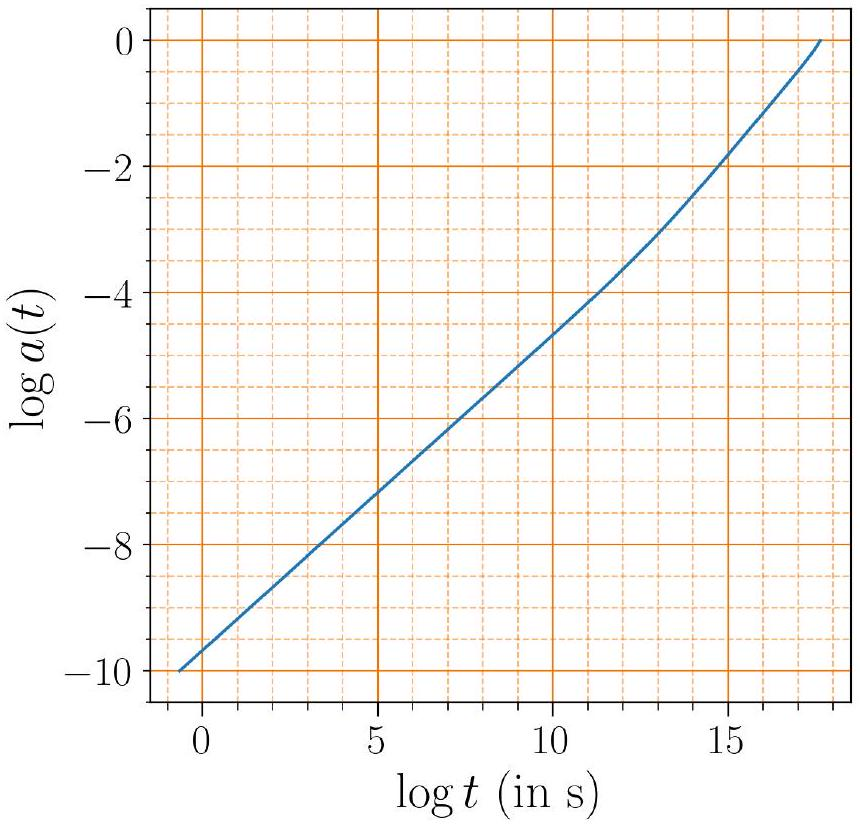
\includegraphics[max width=\textwidth, center]{2025_08_23_e94579452776a99c4850g-19}
    
    If a photon with an energy of $E_{\text {det }}=3.0 \times 10^{20} \mathrm{eV}$ is observed on Earth, determine the largest and the smallest possible values of the initial mass of the PBH ( $M_{0}^{\text {max }}$ and $M_{0}^{\text {min }}$, respectively) which could be responsible for this photon.

\end{document}


\end{document}